\documentclass[9pt]{beamer}

%----- Beamer Theme
\usetheme{Berkeley}
\usecolortheme{seagull}

%\setbeamertemplate{footline}[page number]{}
\setbeamertemplate{navigation symbols}{}


\setbeamercolor{block title}{use=structure,fg=white,bg=red!90!black}
\setbeamercolor{block body}{use=structure,fg=black,bg=red!5!white}

%---- Package
\usepackage{graphicx} % Allows including images
\usepackage{booktabs} % Allows the use of \toprule, \midrule and \bottomrule in tables
\usepackage{amsmath}
\usepackage{amssymb}
\usepackage{hyperref}
\usepackage{physics}
\usepackage[percent]{overpic}
\usepackage{anyfontsize}
\usepackage{mwe}


%----------------------------------------------------------------------------------------
%	TITLE PAGE
%----------------------------------------------------------------------------------------
\title[EPs in Artificial Lattices \& Hybrid Systems]{Exciton--Polaritons in Artificial Lattices \\and\\ Electron Transport in Bose-Fermi Hybrid Systems} % The short title appears at the bottom of every slide, the full title is only on the title page

\author[M. Sun]{Meng Sun \\
\textcolor{red}{Supervisors:~} Prof. Ivan Savenko \and Prof. Sergej Flach \\} % Your name
\institute[UST \and IBS-PCS] % Your institution as it will appear on the bottom of every slide, may be shorthand to save space
{
University of Science \& Technology \\ % Your institution for the title page
Institute of Basic Science, Center for the Theoretical Physics of Complex System\\
\medskip
\textit{sunmeg.89@gmail.com\\} % Your email address
}
\date{ June 18, 2020 via Zoom\\} % Date, can be changed to a custom date
\logo{
\includegraphics[scale=0.04]{IBS.png}}
\titlegraphic{

\includegraphics[width=0.3\textwidth]{log.png}~
\hspace{0.75cm}

\includegraphics[width=0.3\textwidth]{pcs.png}~
%\vspace{10cm}

\includegraphics[width=0.25\textwidth]{ust.png}~
}

%
\makeatletter
\setbeamertemplate{frametitle}{%
    \nointerlineskip%
    \vskip-\beamer@headheight%
    \vbox to \beamer@headheight{%
      \vfil
      \leftskip=-\beamer@leftmargin%
      \advance\leftskip by0.3cm%
      \rightskip=-\beamer@rightmargin%
      \advance\rightskip by0.3cm plus1fil%
      {\usebeamercolor[fg]{frametitle}
          \usebeamerfont{frametitle}\insertframetitle \hfill \insertframenumber/\inserttotalframenumber \par}% added number
      {\usebeamercolor[fg]{framesubtitle}
           \usebeamerfont{framesubtitle}\insertframesubtitle\par}%
      \vbox{}%
      \vskip-1em%
      \vfil
    }%
  }
\makeatother

\begin{document}

\begin{frame}
\titlepage % Print the title page as the first slide
\end{frame}

\begin{frame}
Overview
%\frametitle{Overview} % Table of contents slide, comment this block out to remove it
\tableofcontents % Throughout your presentation, if you choose to use \section{} and \subsection{} commands, these will automatically be printed on this slide as an overview of your presentation

\end{frame}

%----------------------------------------------------------------------------------------
%	PRESENTATION SLIDES
%----------------------------------------------------------------------------------------

%------------------------------------------------
%------------------------------------------------
\section[EPs in Artifical lattices]{Exciton-Polaritons in Artificial lattices} % Sections can be created in order to organize your presentation into discrete blocks, all sections and subsections are automatically printed in the table of contents as an overview of the talk
%------------------------------------------------
%------------------------------------------------

%------------------------------------------------
\subsection[Introduction]{Introduction} % A subsection can be created just before a set of slides with a common theme to further break down your presentation into chunks
%------------------------------------------------

%\begin{frame}
%\begin{block}{
%\begin{huge}
%Exciton--Polaritons in Artificial Lattices
%\end{huge}}
%\begin{itemize}
%\item Introduction
%\item Application
%\end{itemize}
%\end{block}
%\end{frame}

\begin{frame}
\begin{center}
\begin{Huge}
Exciton--Polaritons in Artificial Lattices
\end{Huge}
\end{center}

{\vspace{1.25cm}
\begin{center}
\begin{LARGE}
Introduction
\end{LARGE}
\end{center}}

\end{frame}

\begin{frame}[t]
\frametitle{Introduction}

$\ket{Polariton}=\alpha \ket{Photon}+\beta \ket{Exciton}$
\begin{columns}

\column{.5\textwidth} % Left column and width
\only<1->{
\begin{figure}
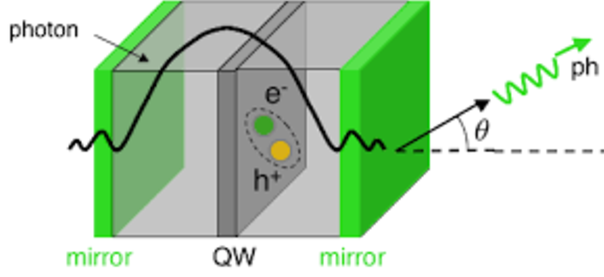
\includegraphics[width=0.75\textwidth]{./fig/cavity.pdf}
\end{figure}}

\only<2->{
A strong coupling between exciton and photon in microcavities
\begin{eqnarray*}
H_{pol}&=&E_{cav}\hat{a}^{\dagger}_k\hat{a}_k+E_{exc}\hat{b}^{\dagger}_k\hat{b}_k\\
&+&\frac{\Omega}{2}\left( \hat{a}^{\dagger}_k\hat{b}_k+\hat{a}_k\hat{b}^{\dagger}_k \right)
\end{eqnarray*}}

\column{.48\textwidth} % Right column and width

\only<3->{
\begin{figure}
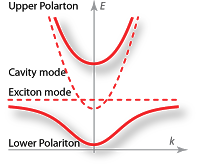
\includegraphics[scale=0.5]{./fig/modes.png}
\end{figure}}

\begin{itemize}
\item<4-> High critical temperature $T_{c}$
\item<5-> Nice coherence properties
\item<6-> Strong Nonlinear interaction
\item<7-> Driven-dissipative system
\item <8-> Detunable
\end{itemize}

\end{columns}
\end{frame}

\begin{frame}
\frametitle{Detuning}
\begin{center}
Detune parameter: $\delta = E_{cav}\left(k=0\right)-E_{exc}\left(k=0\right)$
\end{center}
\begin{figure}
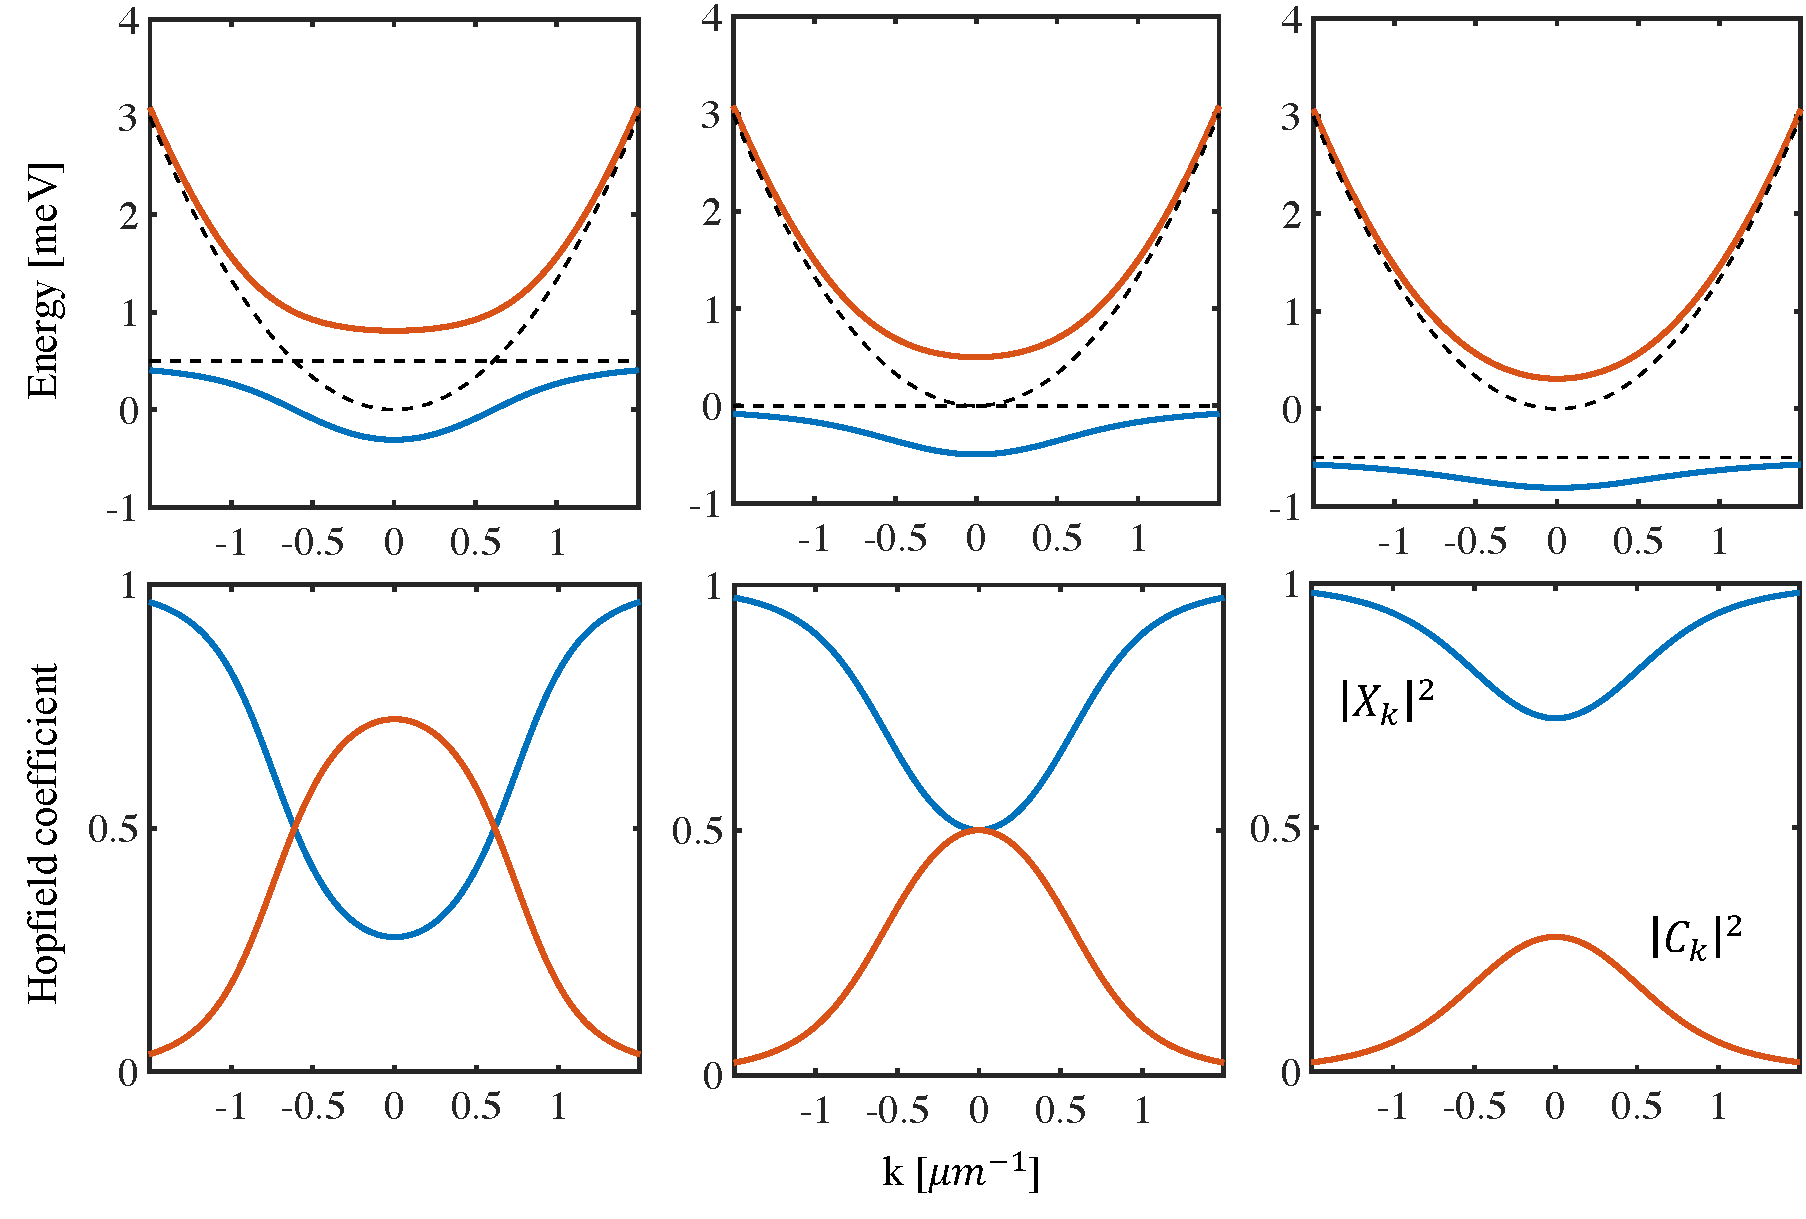
\includegraphics[width=.95\textwidth]{./fig/hp_disp.pdf}
\end{figure}
\end{frame}


\begin{frame}[t]
\frametitle{Artificial Lattice}
\begin{onlyenv}<1-3>
\begin{block}{}<1-3>
With the large scale of de Broglie wavelength, exciton-polaritons can be manipulated by micro-scale potentials.\\
\only<2>{\tiny Pics from \textit{Phys. Rev. B, 93:121303 (2016)}, \textit{Phys. Rev. Lett., 116:066402 (2016)} and \textit{Phys. Rev. Lett., 112:116402 (2014)}.}
\end{block}
\end{onlyenv}

\begin{onlyenv}<2>
\begin{center}
\begin{columns}
\column{.5\textwidth}
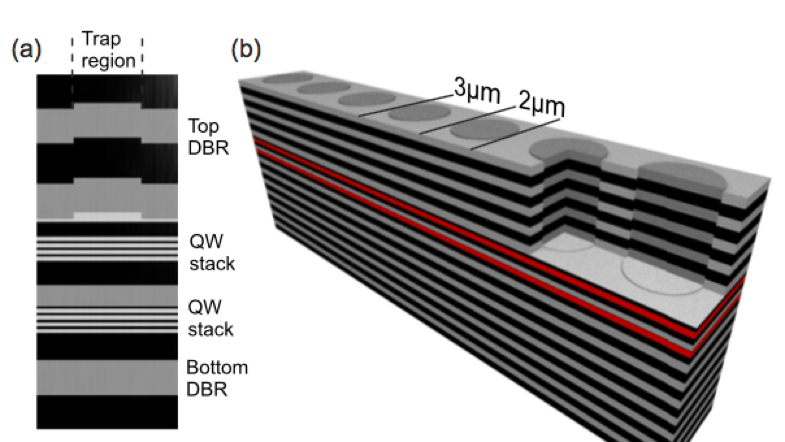
\includegraphics[width=0.95\textwidth]{./fig/lattice0.png}\\
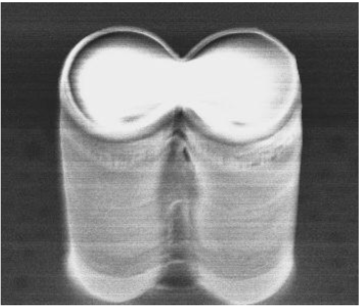
\includegraphics[width=0.44\textwidth]{./fig/twowell.png}
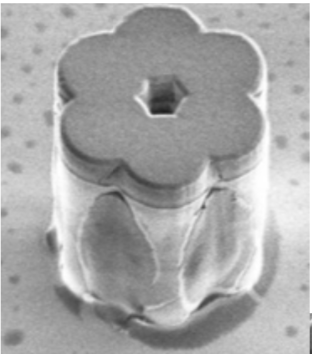
\includegraphics[width=0.44\textwidth]{./fig/bentz.png}
\column{.5\textwidth}
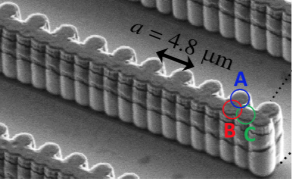
\includegraphics[width=0.825\textwidth]{./fig/lattice2.png}\\
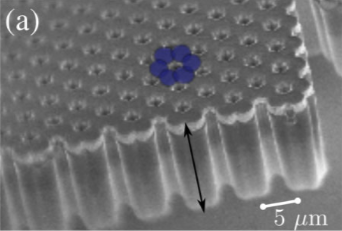
\includegraphics[width=0.825\textwidth]{./fig/lattice1.png}\\
%{\tiny Pic from \cite{Winkler:2016aa},\cite{Baboux:2016aa} and \cite{Jacqmin:2014aa}.}
\end{columns}
\end{center}
\end{onlyenv}

\begin{center}
\begin{block}{Works Include:}<3->
\begin{itemize}
\item Multivalley condensation~\cite{Sun:2017ab}
\item Phase selection and solitons~\cite{Yoon:2019aa}
\item Flat band condensation~\cite{Sun:2018aa,Ko:20}
\item Topological insulator~\cite{Sun:2019ab}
\end{itemize}
\end{block}
\end{center}

\begin{block}{The driven-dissipative Gross--Pitaevskii equation:}<4->
\begin{eqnarray}
        i\hbar \frac{\partial}{\partial t} \psi\left(\mathbf{r},t\right) &=& \left[ -\frac{\hbar^2}{2m}\nabla^2 + V\left(\mathbf{r}\right) + \alpha \abs{\psi\left(\mathbf{r},t\right)}^2 -\frac{i \gamma}{2} \right] \psi\left(\mathbf{r},t\right)\nonumber \\ &+& \frac{i}{2}R\eta_R\left(\mathbf{r},t\right) \psi\left(\mathbf{r},t\right)+ iP\left(\mathbf{r},t\right), \nonumber\\
        \frac{\partial}{\partial t} \eta_R\left(\mathbf{r},t\right) &=& I\left(\mathbf{r},t\right) - R \eta_R\left(\mathbf{r},t\right) \abs{\psi\left(\mathbf{r},t\right)}^2 - \gamma_R \eta_R \left(\mathbf{r},t\right).\nonumber
\end{eqnarray}
\end{block}
\end{frame}


\begin{frame}[t]
\frametitle{The driven-dissipative Gross--Pitaevskii equation}
\begin{onlyenv}<1-4>

\only<1>{\begin{eqnarray}
 i\hbar \frac{\partial}{\partial t} \psi\left(\mathbf{r},t\right) &=& \left[ -\frac{\hbar^2}{2m}\nabla^2 + V\left(\mathbf{r}\right) + \alpha \abs{\psi\left(\mathbf{r},t\right)}^2  \right] \psi\left(\mathbf{r},t\right)\nonumber \\
\nonumber \\
\nonumber
\end{eqnarray}}


\only<2>{\begin{eqnarray}
 i\hbar \frac{\partial}{\partial t} \psi\left(\mathbf{r},t\right) &=& \left[ -\frac{\hbar^2}{2m}\nabla^2 + V\left(\mathbf{r}\right) + \alpha \abs{\psi\left(\mathbf{r},t\right)}^2   \textcolor{red}{-\frac{i \gamma}{2}} \right] \psi\left(\mathbf{r},t\right)\nonumber \\
\nonumber \\
\nonumber
\end{eqnarray}}

\only<3>{\begin{eqnarray}
 i\hbar \frac{\partial}{\partial t} \psi\left(\mathbf{r},t\right) &=& \left[ -\frac{\hbar^2}{2m}\nabla^2 + V\left(\mathbf{r}\right) + \alpha \abs{\psi\left(\mathbf{r},t\right)}^2   -\frac{i \gamma}{2} \right] \psi\left(\mathbf{r},t\right)+\textcolor{red}{iP\left(\mathbf{r},t\right)}\nonumber \\
\nonumber \\
\nonumber
\end{eqnarray}}

\only<4>{\begin{eqnarray}
        i\hbar \frac{\partial}{\partial t} \psi\left(\mathbf{r},t\right) &=& \left[ -\frac{\hbar^2}{2m}\nabla^2 + V\left(\mathbf{r}\right) + \alpha \abs{\psi\left(\mathbf{r},t\right)}^2 -\frac{i \gamma}{2} \right] \psi\left(\mathbf{r},t\right)\nonumber \\ &+& \textcolor{red}{\frac{i}{2}R\eta_R\left(\mathbf{r},t\right) \psi\left(\mathbf{r},t\right)}+iP\left(\mathbf{r},t\right),\nonumber \\
	        \textcolor{red}{\frac{\partial}{\partial t} \eta_R\left(\mathbf{r},t\right)} &=& \textcolor{red}{I\left(\mathbf{r},t\right) - R \eta_R\left(\mathbf{r},t\right) \abs{\psi\left(\mathbf{r},t\right)}^2 - \gamma_R \eta_R \left(\mathbf{r},t\right)}.\nonumber
\end{eqnarray}}

\end{onlyenv}

\begin{onlyenv}<1-4>
\begin{center}
\includegraphics<1>[width=0.45\textwidth]{./fig/gp1.pdf}
\includegraphics<2>[width=0.45\textwidth]{./fig/gp2.pdf}
\includegraphics<3>[width=0.45\textwidth]{./fig/gp3.pdf}
\includegraphics<4>[width=0.45\textwidth]{./fig/gp4.pdf}
\end{center}
\end{onlyenv}
\end{frame}

%-------------------------------------------------
\subsection[Phase selsection]{Phase selection and Solitons}
%-------------------------------------------------

\begin{frame}
\begin{center}
\begin{Huge}
Exciton--Polaritons in Artificial Lattices
\end{Huge}
\end{center}

{\vspace{1.25cm}
\begin{center}
\begin{LARGE}
Phase Selection and Solitons~\cite{Yoon:2019aa}
\end{LARGE}
\end{center}}
\end{frame}

%\begin{frame}
%\begin{block}{
%\begin{huge}
%Phase Selection and soliton
%\end{huge}}
%\begin{itemize}
%%\item Complex valued potential and interaction
%\item Phase selection of condensates
%\item Dark solition behaviour
%\end{itemize}
%\end{block}
%\end{frame}

\begin{frame}[t]
\frametitle{Model}
\only<1->{
\begin{block}{}
\begin{equation}
    i\hbar\partial_t\psi =
    -\frac{\hbar^2}{2 m^*}\partial^2_x\psi + V\left(x\right)\psi
    +\left(\alpha- i\beta\right)|\psi|^2\psi \nonumber
\end{equation}
\end{block}}
\begin{onlyenv}<2->
\begin{center}
\includegraphics<2>[width=.9\textwidth]{./fig/ch3_1.pdf}
\end{center}
\end{onlyenv}
\end{frame}

\begin{frame}[t]
\frametitle{Phase selection}
\only<1->{
\begin{block}{$\Lambda\Lambda$-type}
\begin{equation}
\frac{\alpha}{\beta}=0 ~ ~ ~ ~ ~ ~ ~ ~ ~ \frac{\alpha}{\beta}=2 ~ ~ ~ ~ ~ ~ ~ ~ ~ \frac{\alpha}{\beta}=6 \nonumber
\end{equation}
\end{block}}
\begin{onlyenv}<2->
\begin{center}
\includegraphics<2>[width=1.\textwidth]{./fig/ch3_2.pdf}
\end{center}
\end{onlyenv}
\end{frame}

\begin{frame}[t]
\frametitle{Solitons}
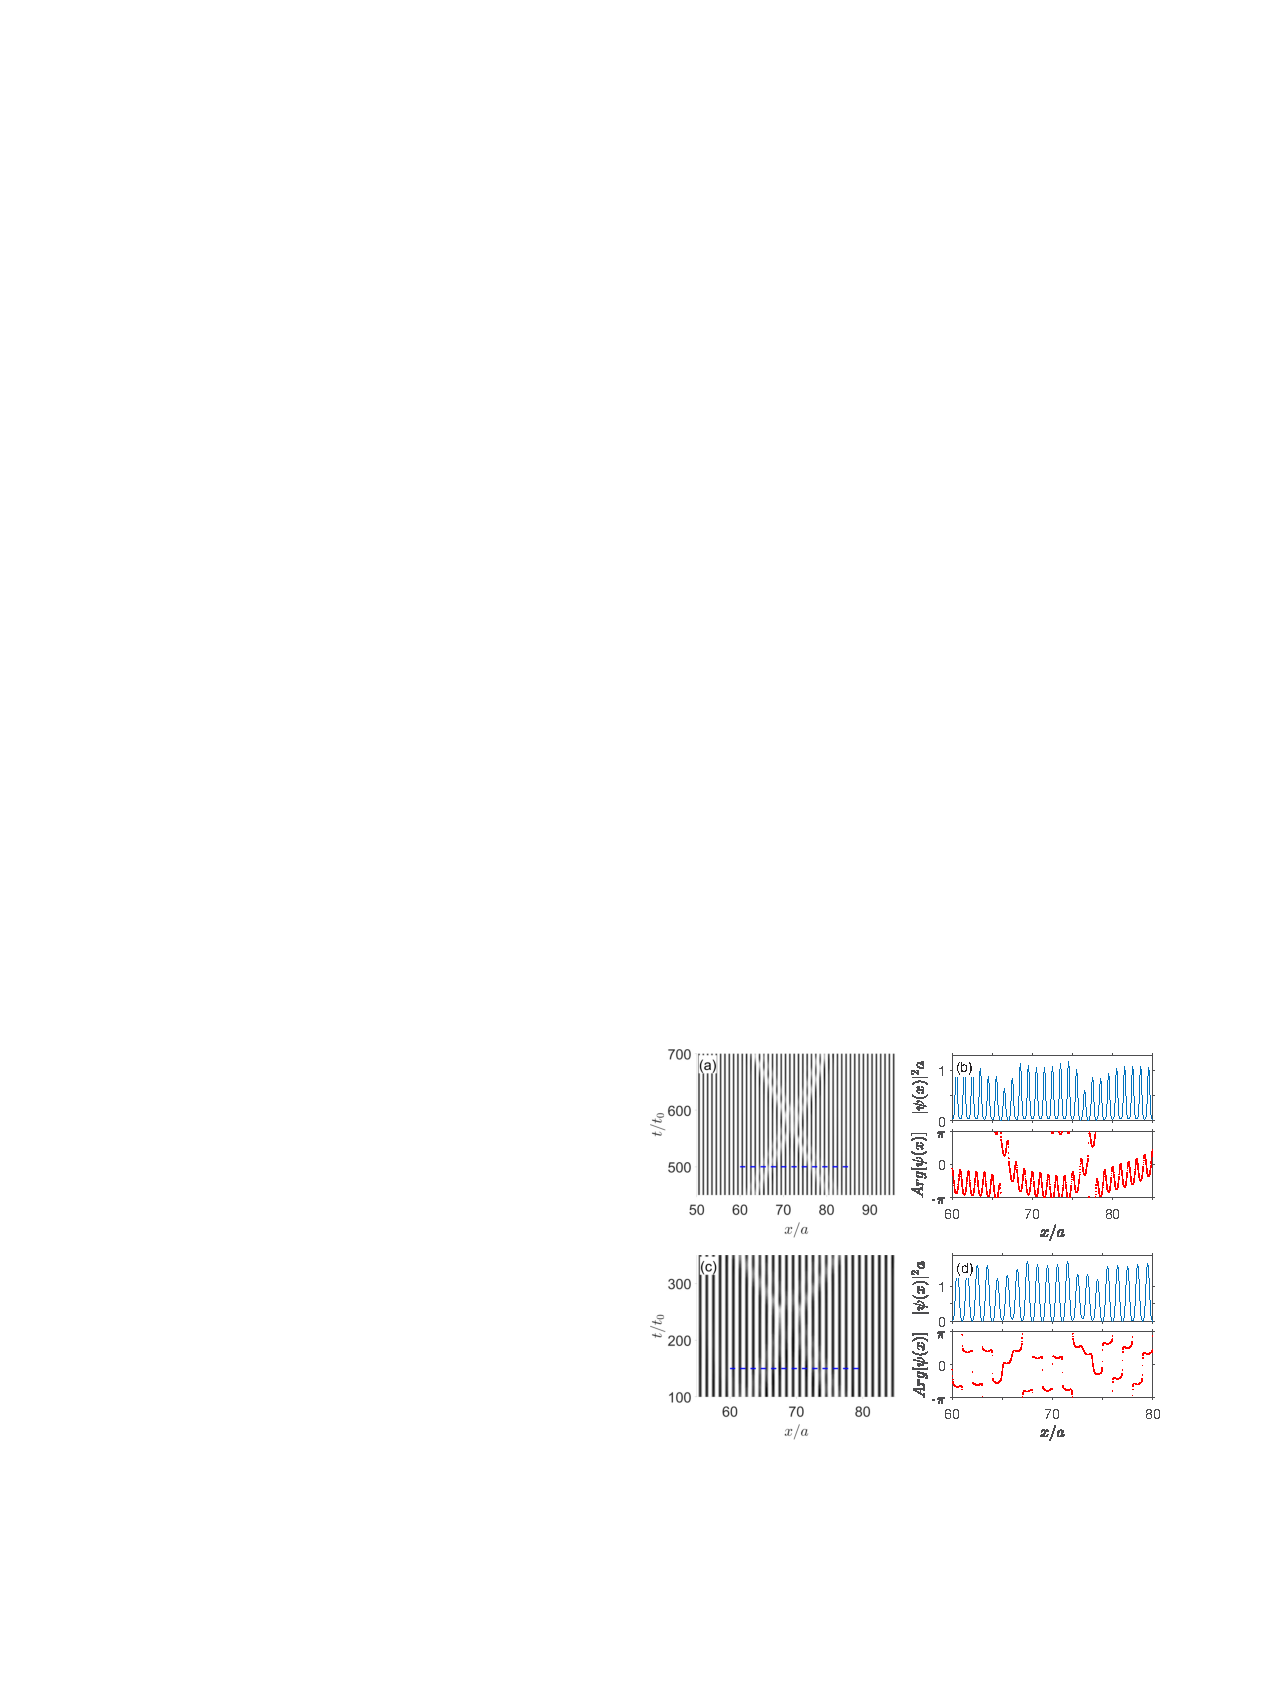
\includegraphics[width=.95\textwidth]{./fig/ch3_4.pdf}
\end{frame}

%\begin{frame}[t]
%\frametitle{Spatiotemporal Intermittency}
%
%\begin{block}{Spatiotemporal intermittency}
%\begin{itemize}
%\item Separate the 0-state and $\pi$-state
%\item Power-law behavior for the distribution of the length of defect domains
%\end{itemize}
%\end{block}
%
%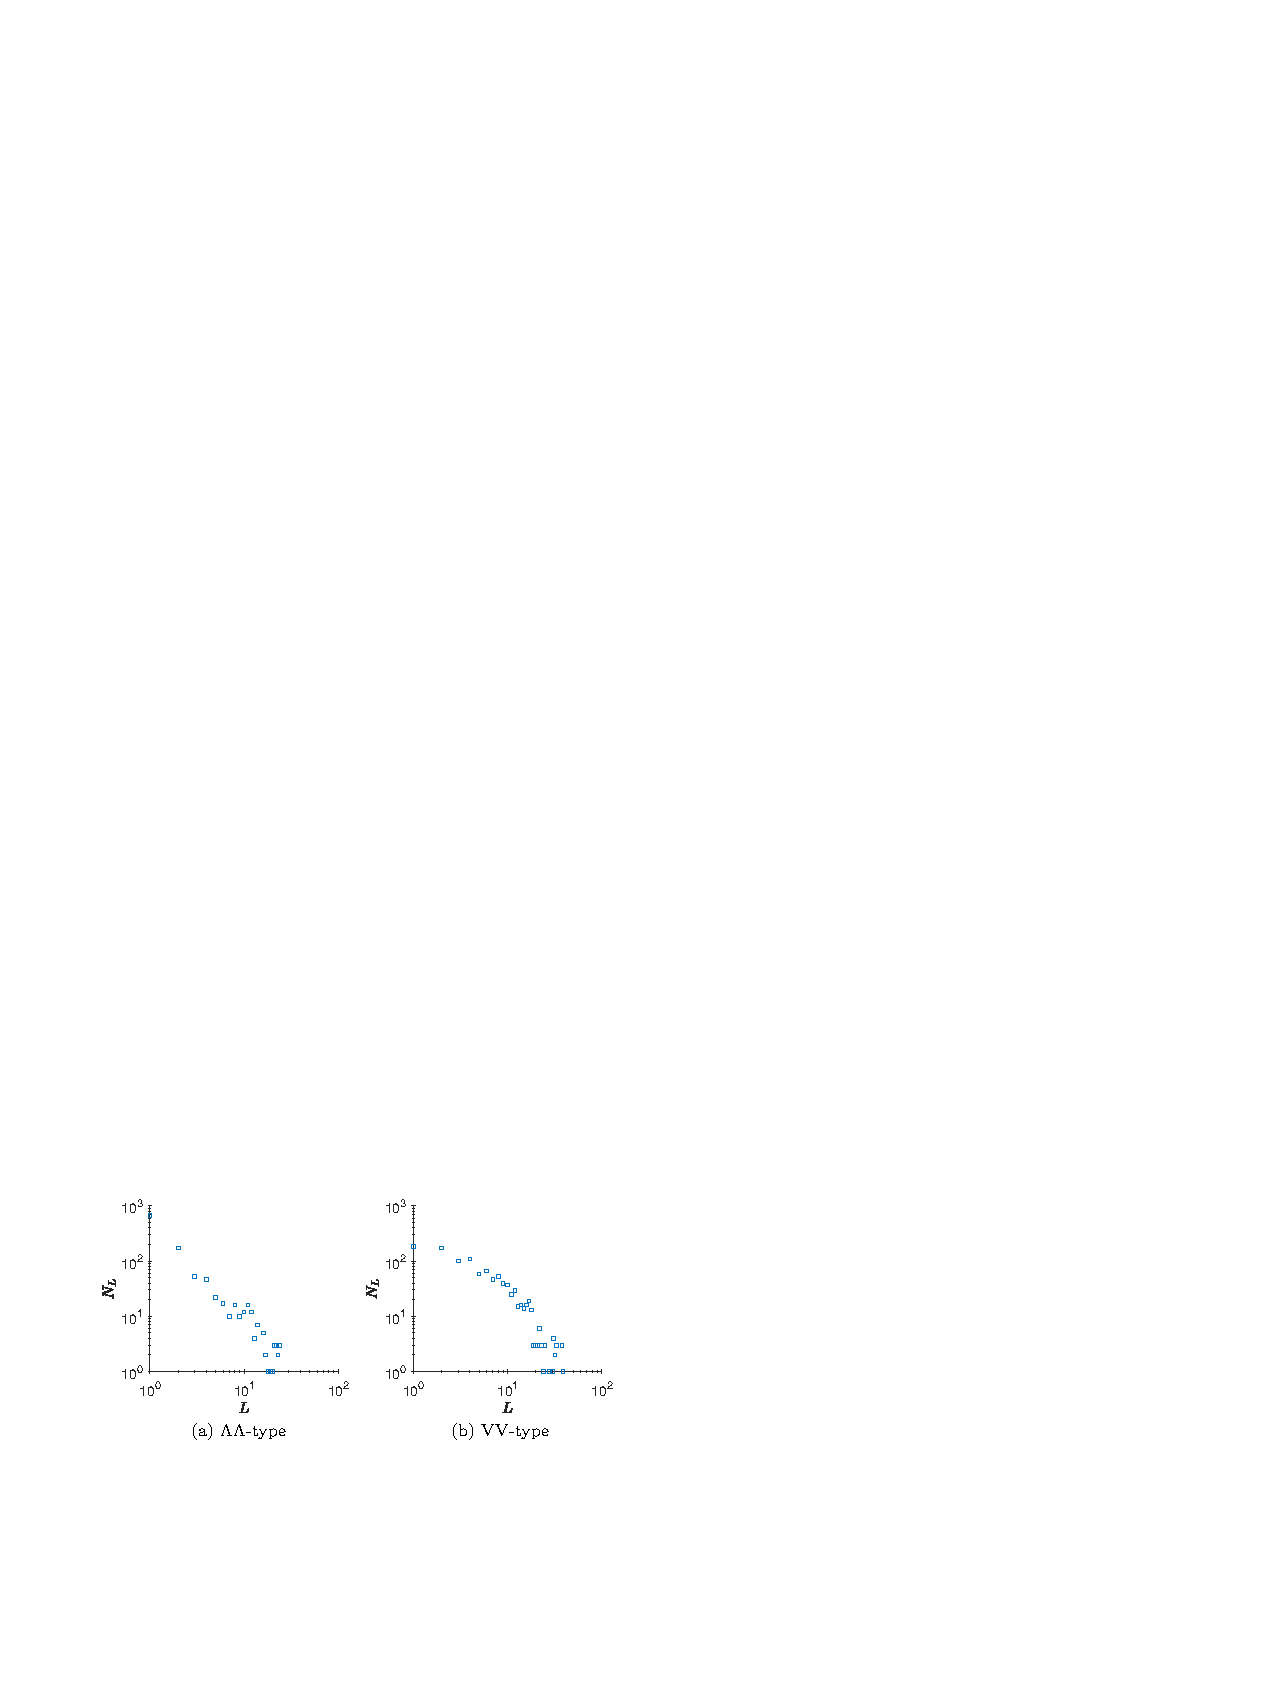
\includegraphics[width=1.\textwidth]{./fig/ch3_3.pdf}
%\end{frame}



%-------------------------------------------------
\subsection[Localized condensates]{Localized condensates in Lieb lattice }
%-------------------------------------------------

\begin{frame}
\begin{center}
\begin{Huge}
Exciton--Polaritons in Artificial Lattices
\end{Huge}
\end{center}

{\vspace{1.25cm}
\begin{center}
\begin{LARGE}
Localiezd condensates in Lieb lattice~\cite{Sun:2018aa}
\end{LARGE}
\end{center}}
\end{frame}

%\begin{frame}
%\begin{block}{
%\begin{huge}
%Excitation of Localized Condensates in Lieb Lattice
%\end{huge}}
%\begin{itemize}
%%\item Exciton-polariton in Lieb lattice
%\item Generate the localized condensate
%\item Maintain the localized condensate
%\end{itemize}
%\end{block}
%\end{frame}

\begin{frame}[t]
\frametitle{Lieb lattice}
\only<2->{
\begin{equation}
\hat{H}=
  \begin{pmatrix}
  -\frac{\nabla^2}{2m_c}+V(\mathbf{r}) & \Omega \\
  \Omega & \delta -\frac{i}{2\tau_x} -\frac{\nabla^2}{2m_x}+\alpha_x|\chi|^2 \nonumber
  \end{pmatrix}
\end{equation}
}

\only<1->{
\begin{center}
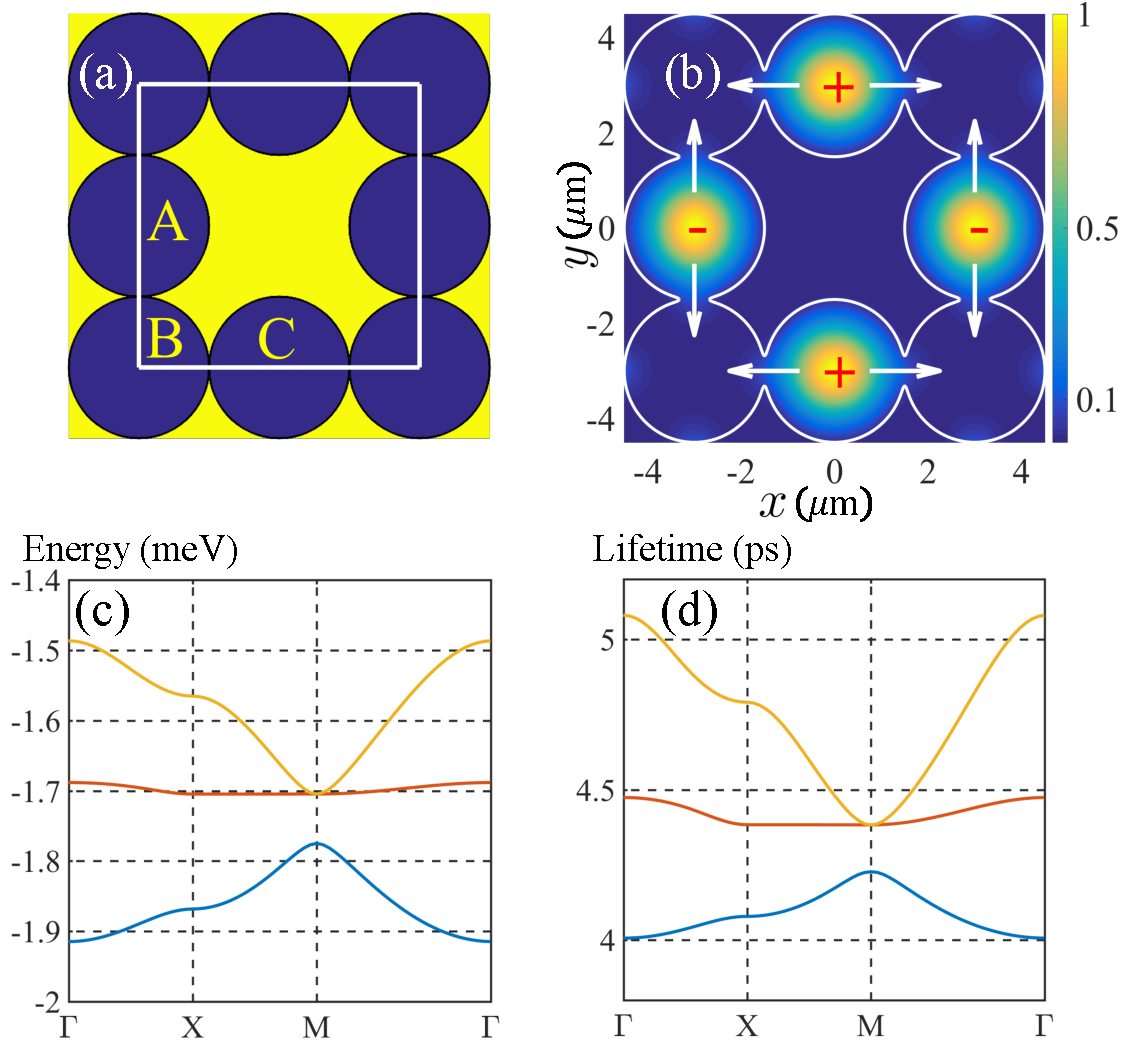
\includegraphics[width=.55\textwidth]{./fig/ch4_1.pdf}
\end{center}
}

\end{frame}

\begin{frame}[t]
\frametitle{Laguerre--Gaussian resonant pumping}
\only<1-2>{
\begin{equation}
  P(\mathbf{r},t)=P_0 \frac{(x\pm{i}y)^2}{R^2}
  \exp\!\left[-\frac{r^2}{R^2}-i\omega_0t\right]\!\theta(t)\theta(t_p-t). \nonumber
\end{equation}}

\only<3->{
\begin{equation}
i\begin{pmatrix}\dot{\varphi}\\\dot{\chi}\end{pmatrix} =
 \hat{H}\begin{pmatrix}{\varphi}\\{\chi}\end{pmatrix}
% +\frac{{i}cn_r}{2}\begin{pmatrix}{0}\\{\chi}\end{pmatrix}
 +\begin{pmatrix}{iP(\mathbf{r},t)}\\{0}\end{pmatrix}.  \nonumber
\end{equation}}

\begin{center}
\includegraphics<2-3>[width=0.45\textwidth]{./fig/ch4_2.pdf}
\includegraphics<4->[width=0.45\textwidth]{./fig/ch4_3.pdf}
\end{center}
\end{frame}


\begin{frame}[t]
\frametitle{Prolonging the condensate}
\begin{subequations}\label{CH3_INC}
\begin{align}
 i\begin{pmatrix}\dot{\varphi}\\\dot{\chi}\end{pmatrix} &=
 \hat{H}\begin{pmatrix}{\varphi}\\{\chi}\end{pmatrix}
 +\frac{{i}cn_r}{2}\begin{pmatrix}{0}\\{\chi}\end{pmatrix}
 +\begin{pmatrix}{iP(\mathbf{r},t)}\\{0}\end{pmatrix},  \nonumber \\
 \frac{\partial n_r}{\partial t} &= I - \tau_r^{-1} n_r-c|\chi|^2n_r. \nonumber
\end{align}
\end{subequations}
\begin{center}
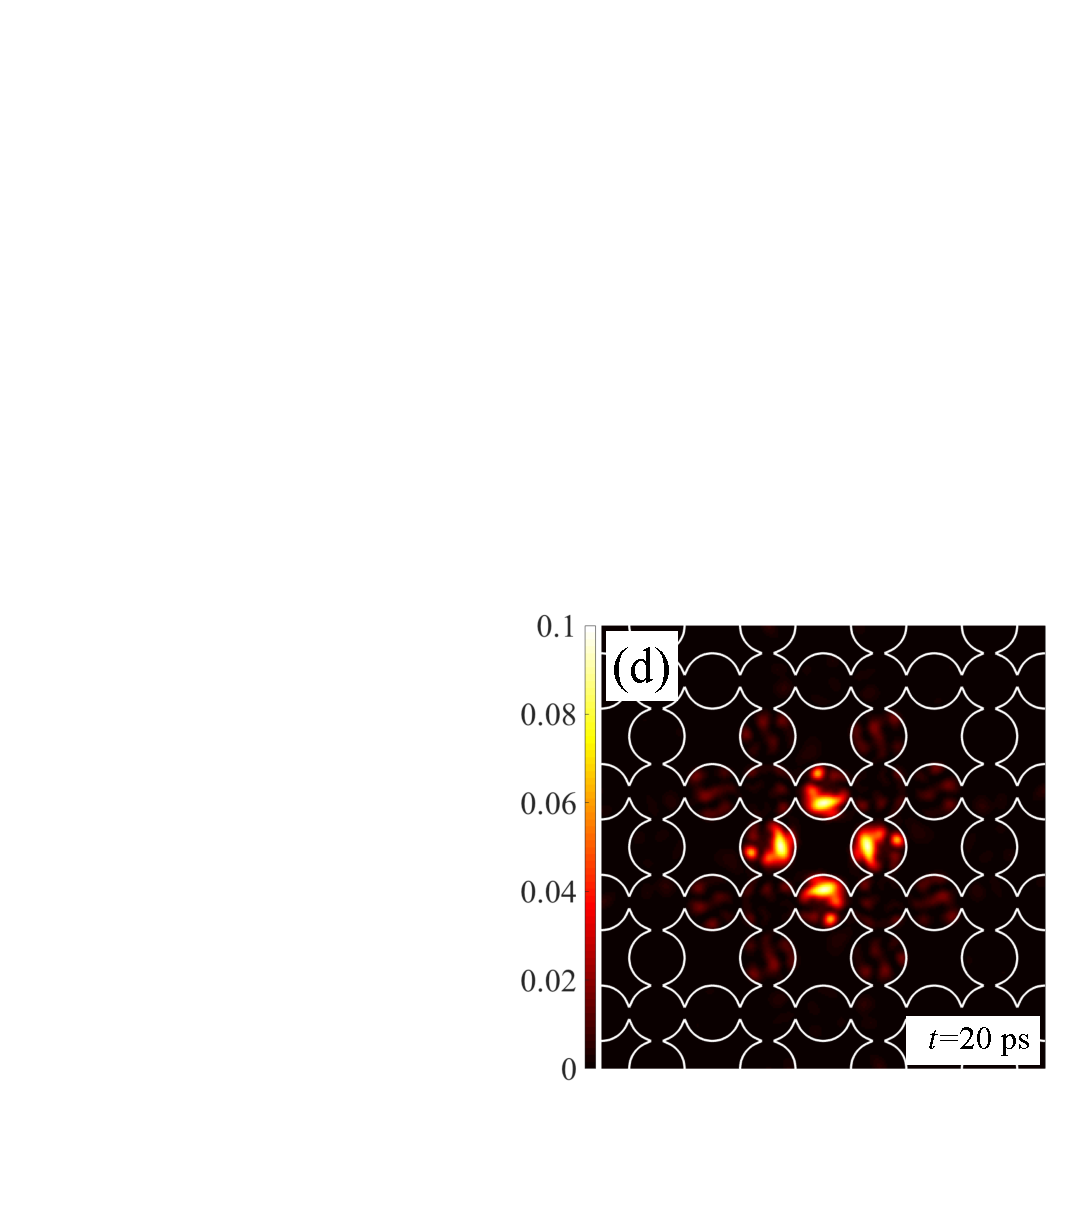
\includegraphics[width=0.45\textwidth]{./fig/prolong.pdf}
\end{center}
\end{frame}

%------------------------------------------------
%-------------------------------------------------
\section[Hybrid system]{Electron Transport in Bose-Fermi Hybrid Systems}
%-------------------------------------------------
%------------------------------------------------

\begin{frame}
\begin{center}
\begin{Huge}
Electron Transport in Bose-Fermi Hybrid Systems
\end{Huge}
\end{center}

{\vspace{1.25cm}
\begin{center}
\begin{LARGE}
Bogolon--Mediated Electron Scattering~\cite{Sun:2019aa,Villegas:2019aa}
\end{LARGE}
\end{center}}
\end{frame}

%\begin{frame}
%\begin{block}{
%\begin{huge}
%Bogolon--Mediated Electron Scattering in Hybrid System~\cite{Sun:2019aa,Villegas:2019aa}
%\end{huge}}
%\begin{itemize}
%\item Electron-bogolon interaction
%\item Resistivity as a function of temperature
%\end{itemize}
%\end{block}
%\end{frame}

%------------------------------------------------
\subsection[System setting]{System setting}
%------------------------------------------------
\begin{frame}[t]
\frametitle{Hybrid Bose-Fermi system}
\begin{onlyenv}<1-3>
\begin{block}{}
\only<1-2>{\begin{itemize}
\item A layer of fermions (graphene or normal metal)
\item A layer of bosons in condensate (indirect-exciton)
\item Columb interaction between fermion and boson layers
\end{itemize}}
\only<3>{\begin{eqnarray}
g\left(r\right) &=& \frac{e_0^2}{4\pi\epsilon}\left( \frac{1}{r_{ee}}-\frac{1}{r_{eh}}\right) \nonumber \\
g\left(k\right) &=&  \frac{e_0^2}{2 k \epsilon } e^{-kl} \left( 1 - e^{-kd} \right) \nonumber
\end{eqnarray}}
\end{block}
\only<2->{
\begin{center}
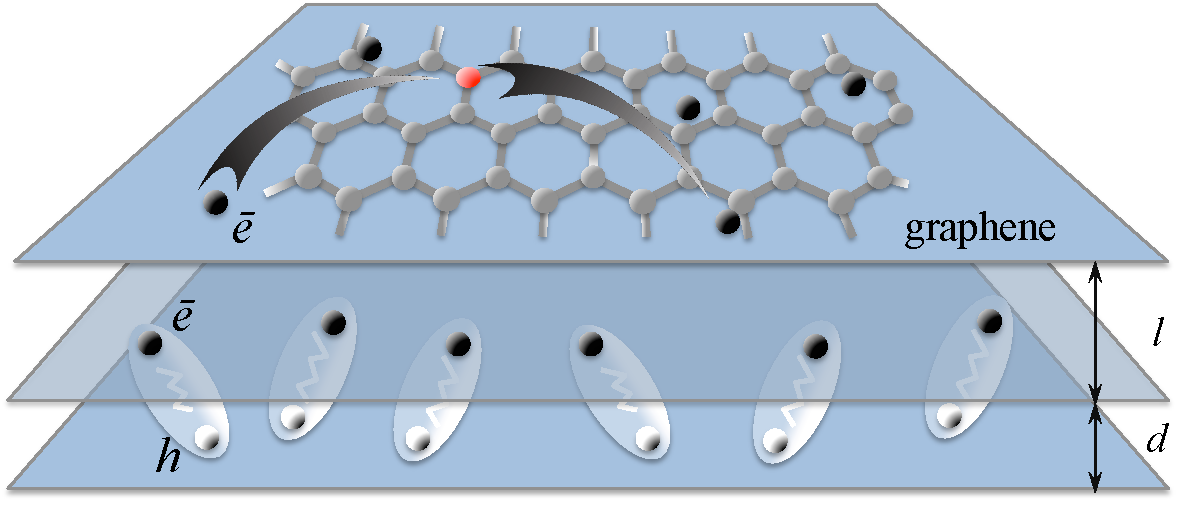
\includegraphics[width=0.75\textwidth]{./fig/ch6_1.pdf}
\end{center}}
\end{onlyenv}
\end{frame}

\begin{frame}[t]
\frametitle{Interaction terms}
\begin{onlyenv}<1->
\only<1-3>{
\begin{block}{Electron-exciton interaction}
\begin{equation}
V=\int d\mathbf{r}\int d\mathbf{R}\Psi^\dag_\mathbf{r}\Psi_\mathbf{r}g\left(\mathbf{r}-\mathbf{R}\right)\Phi^\dag_\mathbf{R}\Phi_\mathbf{R}\nonumber
\end{equation}
\end{block}}
\end{onlyenv}

\begin{onlyenv}<1->
\setbeamercolor{block title}{use=structure,fg=white,bg=black!25!white}
\setbeamercolor{block body}{use=structure,fg=black,bg=black!5!white}
\only<2-3>{
\begin{block}{Exictons in BEC}
\begin{equation}
\Phi_\mathbf{R} = \sqrt{n_c} + \phi_\mathbf{R} \nonumber
\end{equation}
\end{block}}
%
\only<4-5>{
\begin{block}{Bogoliubov transformation}
%\begin{equation}
%\varphi^\dag_\mathbf{R}+\varphi_\mathbf{R}=\sum_{\mathbf{p}} e^{i\mathbf{pR}} \left[(u_\mathbf{p}+v_{-\mathbf{p}})b_\mathbf{p}+(v_\mathbf{p}+u_{-\mathbf{p}})b^\dag_{-\mathbf{p}}\right] \nonumber
%\end{equation}
\begin{equation}
\phi_p = u_p b_p + v_p b^\dagger_{-p},~ ~ \phi_p^\dagger = u_p b_p^\dagger + v_p b_{-p} \nonumber
\end{equation}
\begin{equation*}
u_p^2 = 1+v_p^2 = \frac{1}{2} \left( 1 + \sqrt{1+ \frac{M^2 s^4}{\omega_p^2}}\right), ~ ~ u_p v_p = -\frac{Ms^2}{2\omega_p}
\end{equation*}
\end{block}}
\end{onlyenv}

\begin{onlyenv}<1->
\only<3>{
\begin{block}{}
\begin{eqnarray}
V_1 &=& \sqrt{n_c}\int d\mathbf{r}\Psi^\dag_\mathbf{r}\Psi_\mathbf{r} \int d\mathbf{R}g\left(\mathbf{r}-\mathbf{R}\right)\left[\phi^\dag_\mathbf{R}+\phi_\mathbf{R}\right] \nonumber \\
V_2 &=& \int d\mathbf{r} \Psi^\dagger_\mathbf{r} \Psi_\mathbf{r} \int d\mathbf{R} g\left(\mathbf{r}-\mathbf{R}\right) \phi^\dagger_\mathbf{R} \phi_\mathbf{R} \nonumber
\end{eqnarray}
\end{block}}
%
\only<5>{
\begin{block}{One- and two-bogolon interaction}
\begin{eqnarray}
V^{(1)} &=& \frac{\sqrt{n_c}}{L} \sum_{\mathbf{k,p}} g_\mathbf{p} \left[ \left( v_\mathbf{p} + u_\mathbf{-p} \right)b^\dagger_\mathbf{-p} + \left( u_\mathbf{p} + v_\mathbf{-p}\right)b_\mathbf{p} \right] c^\dagger_\mathbf{k+p} c_\mathbf{k} \nonumber \\
V^{(2)} &=& \frac{1}{L^2}\sum_{\mathbf{k},\mathbf{p},\mathbf{q}} g_\mathbf{p}\bigg[ u_{\mathbf{q}-\mathbf{p}} u_\mathbf{q} b^\dagger_{\mathbf{q}-\mathbf{p}} b_\mathbf{q} + u_{\mathbf{q}-\mathbf{p}} v_\mathbf{q} b^\dagger_{\mathbf{q}-\mathbf{p}} b^\dagger_{-\mathbf{q}} \nonumber \\
&+& v_{\mathbf{q}-\mathbf{p}} u_\mathbf{q} b_{-\mathbf{q}+\mathbf{p}} b_\mathbf{q} + v_{\mathbf{q}-\mathbf{p}} v_\mathbf{q} b_{-\mathbf{q}+\mathbf{p}} b^\dagger_{-\mathbf{q}}\bigg] c^\dagger_{\mathbf{k}+\mathbf{p}} c_\mathbf{k} \nonumber
\end{eqnarray}
\end{block}}
\end{onlyenv}
\only<6>{
\begin{center}
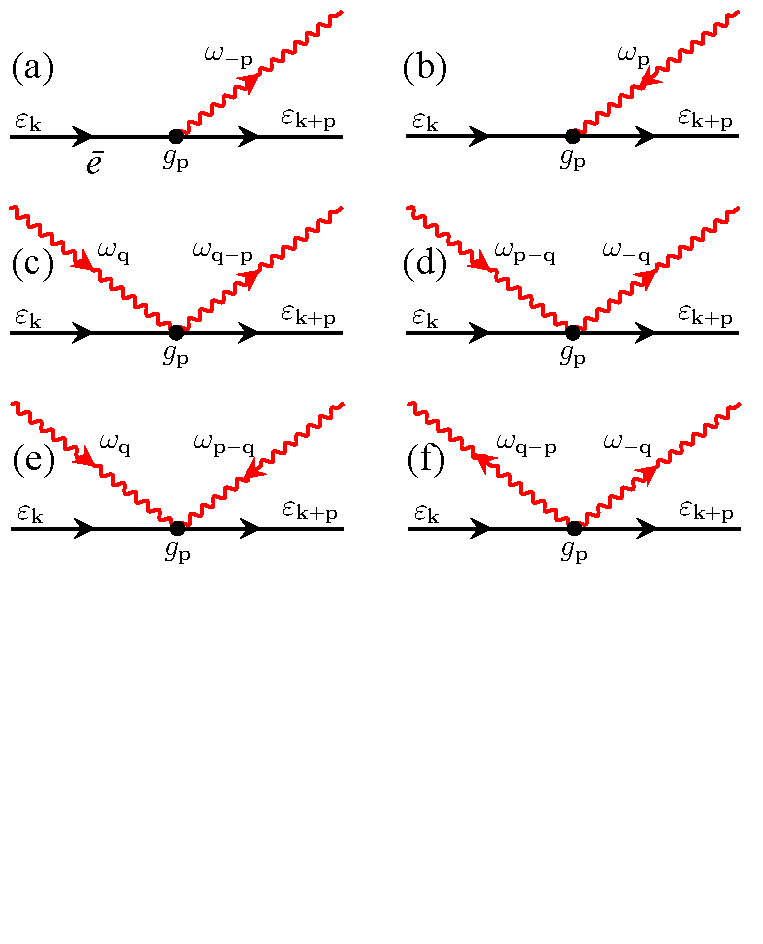
\includegraphics[width=0.85\textwidth]{./fig/ch6_2.pdf}
\end{center}}
\end{frame}

%------------------------------------------------
\subsection[Theory]{Bloch--Gr\"{u}neisen approach for resistivity}
%------------------------------------------------
\begin{frame}[t]
\frametitle{Bloch--Gr\"{u}neisen approach for resistivity}
\begin{onlyenv}<1->
\begin{block}{Boltzmann equation}
\only<1->{
\begin{equation}
%\frac{df\left(\mathbf{r},\mathbf{p},t\right)}{dt}=\textcolor{red}{\frac{\partial f}{\partial t}}+\textcolor{red}{\frac{\partial f}{\partial \mathbf{r}}}\frac{d\mathbf{r}}{dt}
%+\frac{\partial f}{\hbar\partial \mathbf{p}}\frac{\hbar d\mathbf{p}}{dt} \nonumber
e_0 \mathbf{E} \frac{\partial f}{\hbar\partial \mathbf{p}} = I\lbrace f \rbrace \nonumber
\end{equation}}
%
%\only<2>{
%\begin{equation}
%\frac{df}{dt}=
%\mathbf{F}\cdot
%\frac{\partial f}{\hbar\partial \mathbf{p}}\nonumber
%\end{equation}}
%
%\only<3->{
%\begin{equation}
%e_0 \mathbf{E} \frac{\partial f}{\hbar\partial \mathbf{p}} = I\lbrace f \rbrace \nonumber
%\end{equation}}
\end{block}

\only<2>{
\begin{block}{Collision integral}
\begin{eqnarray}
\label{AP7_Eq2}
I\{f\}&=&-\frac{1}{\hbar}\int\frac{d\textbf{q}d\textbf{p}'}{(2\pi)^2}|V^{(1)}_q|^2\nonumber \\
&{}&{}\times\Bigl[N_qf_p(1-f_{p'})\delta(\varepsilon_p-\varepsilon_{p'}+\hbar\omega_q)\delta(\textbf{p}-\textbf{p}'+\textbf{q})\nonumber\\
&{}&{}+(N_q+1)f_p(1-f_{p'})\delta(\varepsilon_p-\varepsilon_{p'}-\hbar\omega_q)\delta(\textbf{p}-\textbf{p}'-\textbf{q})\nonumber \\
&{}&{}-N_qf_{p'}(1-f_{p})\delta(\varepsilon_{p'}-\varepsilon_{p}+\hbar\omega_q)\delta(\textbf{p}'-\textbf{p}+\textbf{q})\nonumber\\
&{}&{}-(N_q+1)f_{p'}(1-f_p)\delta(\varepsilon_{p'}-\varepsilon_{p}-\hbar\omega_q)\delta(\textbf{p}'-\textbf{p}-\textbf{q})\Bigr] \nonumber
\end{eqnarray}
\end{block}}

\only<3->{
\begin{onlyenv}<3->
\setbeamercolor{block title}{use=structure,fg=white,bg=black!25!white}
\setbeamercolor{block body}{use=structure,fg=black,bg=black!5!white}
\begin{block}{Weak electric field}
\begin{equation}
f= f^0\left( \varepsilon_p\right)+\left( \frac{\partial f^0}{\partial \varepsilon_p}\right) \phi_p \nonumber
\end{equation}
\begin{equation}
\phi_p = e_0 E_x \tau\left(\varepsilon_p\right)  \frac{\partial \varepsilon_p}{\hbar\partial p_x}\nonumber
\end{equation}
\end{block}
\end{onlyenv}}

\only<4->{
\begin{block}{Resistivity}
\begin{equation}
\rho^{-1} = e_0^2 \mathcal{D}\left(\varepsilon_f\right) \frac{v_f^2}{2} \langle \tau \rangle \nonumber
\end{equation}
\end{block}}
\end{onlyenv}
\end{frame}



%------------------------------------------------
\subsection[Result]{Result}
%------------------------------------------------
\begin{frame}[t]
\frametitle{Linear dispersion: One bogolon process}
\begin{block}{}
\begin{equation}
\rho \propto T^4 ~(T\ll T_{BG}), ~ ~ ~ ~ \rho \propto T^1 ~(T \gg T_{BG})\nonumber
\end{equation}
\begin{equation}
T_{BG} = \frac{2\hbar s k_f}{k_B} \nonumber
\end{equation}
\end{block}
\begin{center}
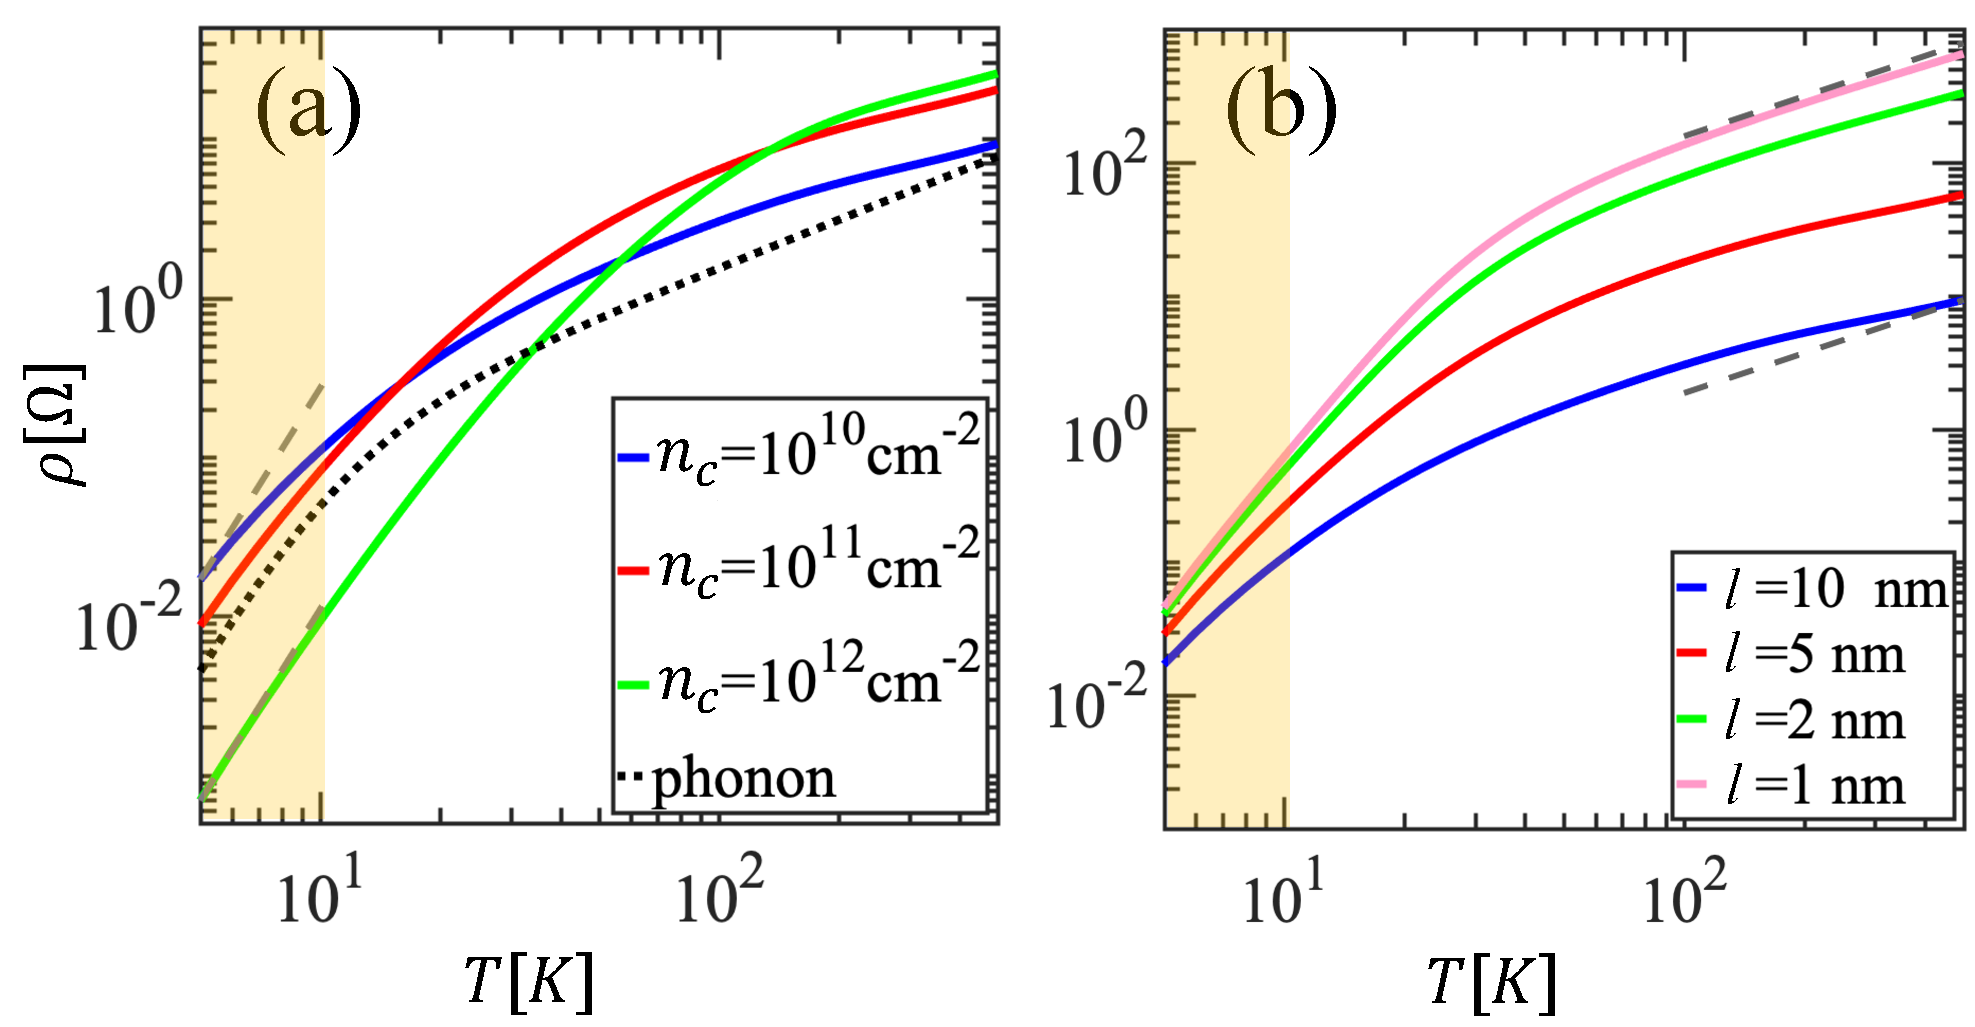
\includegraphics[width=0.9\textwidth]{./fig/ch6_3.pdf}
\end{center}
\end{frame}

\begin{frame}[t]
\frametitle{Parabolic dispersion: One \& two bogolon process}
\begin{center}
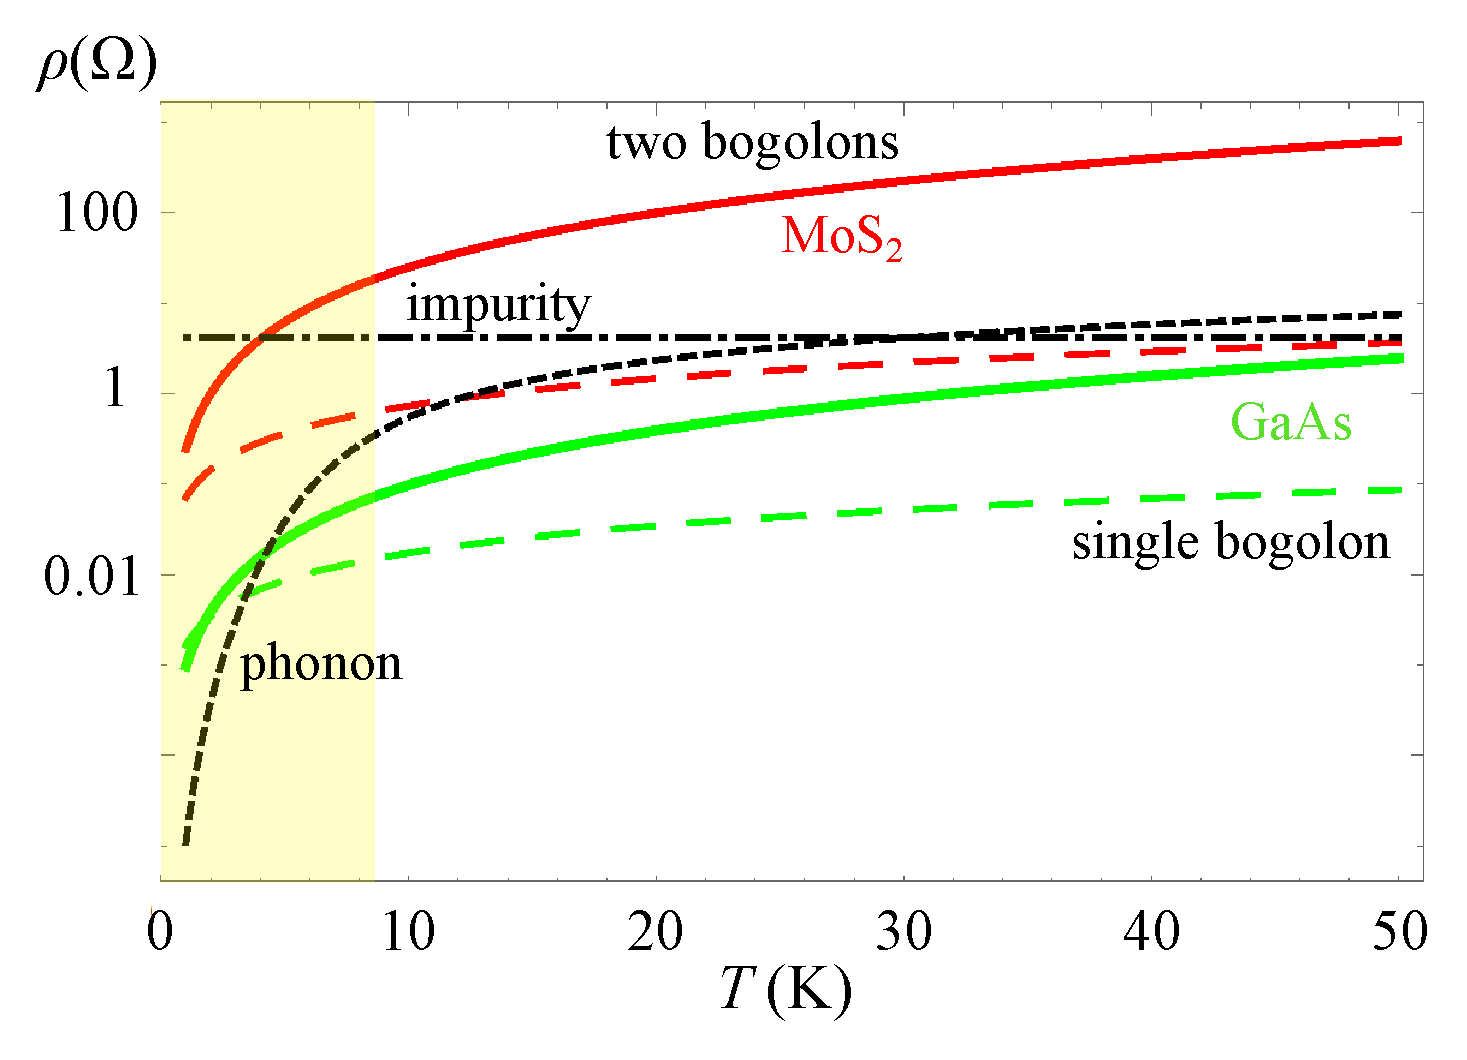
\includegraphics[width=0.75\textwidth]{./fig/ch6_5.pdf}
\end{center}
\end{frame}

%------------------------------------------------
%------------------------------------------------
\section{Summary}
%------------------------------------------------
%------------------------------------------------

\begin{frame}
\frametitle{Summary}
\begin{center}
\begin{block}{Phase selection}
\begin{itemize}
%\item Multivalley condensation
\item Condensate: $0-$phase $\Leftrightarrow$ $\pi-$phase
\item Dark soliton
\end{itemize}
\end{block}
%
\begin{block}{Lieb lattice}
\begin{itemize}
\item Exciton-polariton dispersion in Lieb lattice
\item Excite the CLS
%\item Prolong the CLS
\end{itemize}
\end{block}
%
\begin{block}{Hybrid system}
\begin{itemize}
\item Temperature dependent resistivity
\item Two-bogolon dominant in parabolic case
%\item Topological insulator 
%\item Temperature dependence resistivity result.
\end{itemize}
\end{block}
\end{center}
\end{frame}

\begin{frame}
\frametitle{Publication list}
\scriptsize	
\bibliographystyle{unsrt}
\setbeamertemplate{bibliography item}[text]
\bibliography{Library}
\end{frame}


\begin{frame}
\begin{center}

\includegraphics[width=0.85\textwidth]{./fig/thankyou.pdf}
\end{center}
\end{frame}


\begin{frame}[plain]
\begin{center}

\end{center}
\end{frame}

%%-------------------------------------------------
%\subsection[1-2]{Multivalley engineering}
%%-------------------------------------------------
%
%\begin{frame}
%\begin{block}{
%\begin{huge}
%Multivalley Engineering~\cite{Sun:2017ab}
%\end{huge}}
%\begin{itemize}
%\item Separately manipulation of photon and exciton
%\item Nontrivial ground state condensate
%\item TE-TM splitting 
%\end{itemize}
%\end{block}
%\end{frame}
%
%\begin{frame}[t]
%\frametitle{Multivalley engineering in semiconductor microcavities}
%
%\begin{onlyenv}<1-2>
%\begin{block}{}<1-2>
%\textit{"\dots we consider the behavior of exciton-polaritons in a microcavity where both the optical and excitonic components are separately manipulated by two periodic potentials \dots"}
%\end{block}
%\end{onlyenv}
%
%\begin{onlyenv}<3-4>
%\begin{block}{}<3-4>
%\textit{Considering the model with incoherent pumping}
%{\small
%\begin{eqnarray*}
%	i\hbar\frac{\partial\psi(x,t)}{\partial t} &=& {\cal F}^{-1}\left[E_k\psi_k+{\cal S}_k(t)\right]  +\frac{i\hbar}{2} \left[ R n_{r}(x,t) -\gamma_0-\frac{2i}{\hbar}\alpha |\psi({x},t)|^2 \right]\psi(x,t)\\
%	&+& \sum_k\left[{\cal T}_{-k}(t)+{\cal T}^*_k(t)\right]e^{-ikx}\psi(x,t) \\
%	\frac{\partial n_{r}(x,t)}{\partial t}&=&-(\gamma_{r}+R|\psi(x,t)|^2)n_{r}+P.  
%\end{eqnarray*}
%}
%\end{block}
%\end{onlyenv}
%
%\begin{onlyenv}<5-6>
%\begin{block}{From 1D to 2D}<5-6>
%\begin{eqnarray}
%\label{eq:CH2_TE_TM}
%\mathcal{H}_{TE-TM}=\left(\begin{array}{cc}0&\Delta\left(i\frac{\partial}{\partial x}+\frac{\partial}{\partial y}\right)^2\\\Delta\left(i\frac{\partial}{\partial x}-\frac{\partial}{\partial y}\right)^2&0\end{array}\right). \nonumber
%\end{eqnarray}
%\end{block}
%\end{onlyenv}
%
%\begin{onlyenv}<1-4>
%\begin{center}
%\includegraphics<2>[width=.85\textwidth]{./fig/ch2_1.pdf}
%\includegraphics<4>[width=1.05\textwidth]{./fig/ch2_2.jpg}
%\end{center}
%\end{onlyenv}
%
%\begin{center}
%\includegraphics<6->[width=1.\textwidth]{./fig/ch2_3.jpg}
%\end{center}
%
%\end{frame}

%%-------------------------------------------------
%\subsection[Topological Insulator]{Topological Insulatior with quantum magnetic dots }
%%-------------------------------------------------
%\begin{frame}
%\begin{block}{
%\begin{huge}
%Topological Insulator with Quantum Magnetic dots~\cite{Sun:2019ab}
%\end{huge}}
%\begin{itemize}
%\item Magnetic quantum dots
%\item Edge mode
%\item Phase diagram
%\end{itemize}
%\end{block}
%\end{frame}
%
%\begin{frame}[t]
%\frametitle{Magnetic dots}
%
%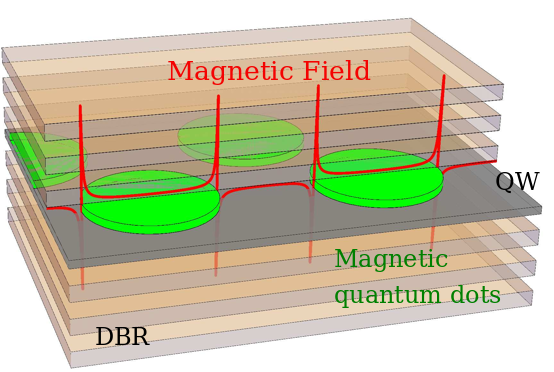
\includegraphics[width=0.6\textwidth]{./fig/ch5_1.png}
%
%\begin{onlyenv}<1-3>
%\only<1>{
%\begin{huge}
%\begin{eqnarray}\label{eq:Ch5_EqDotMF}
%B_z(r,z)=2\pi \mu_0 M R\int_0^\infty J_0(rq)J_1(Rq)\mathrm{e}^{-|z|q}q dq \nonumber
%\end{eqnarray}
%\end{huge}}
%{ \vspace{-0.5in} \hfill \only<2>{
%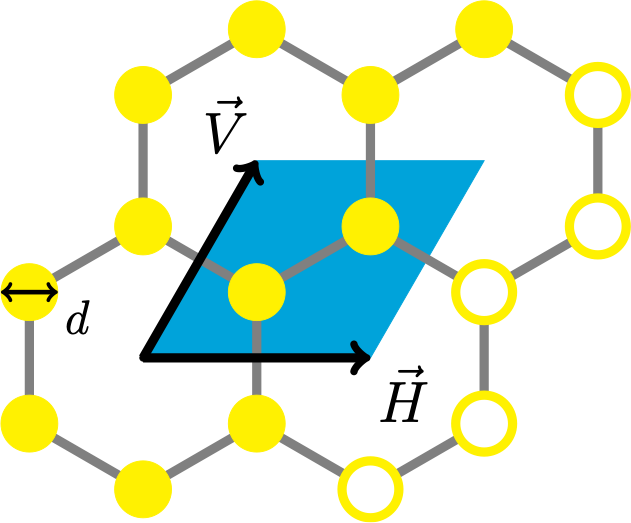
\includegraphics[width=0.5\textwidth]{./fig/ch5_2.png}}}
%{\only<3>{
%	\vspace{0.5in}{
%\begin{Large}
%\begin{eqnarray}
%i\hbar \frac{\partial \psi_{\pm}}{\partial t} &=& -\frac{\hbar^2}{2m_{eff}}\nabla^2 \psi_{\pm} + V \psi_{\pm} + \Delta_{\pm}^{eff} \psi_{\pm} \nonumber \\
%    &+& \beta^{eff} \left( \partial_x \mp i \partial_y \right)^2 \psi_\mp \nonumber
%\end{eqnarray}
%\end{Large}
%}}}
%\end{onlyenv}
%\end{frame}
%
%\begin{frame}[t]
%\frametitle{Edge Mode \& Phase plot}
%\begin{center}
%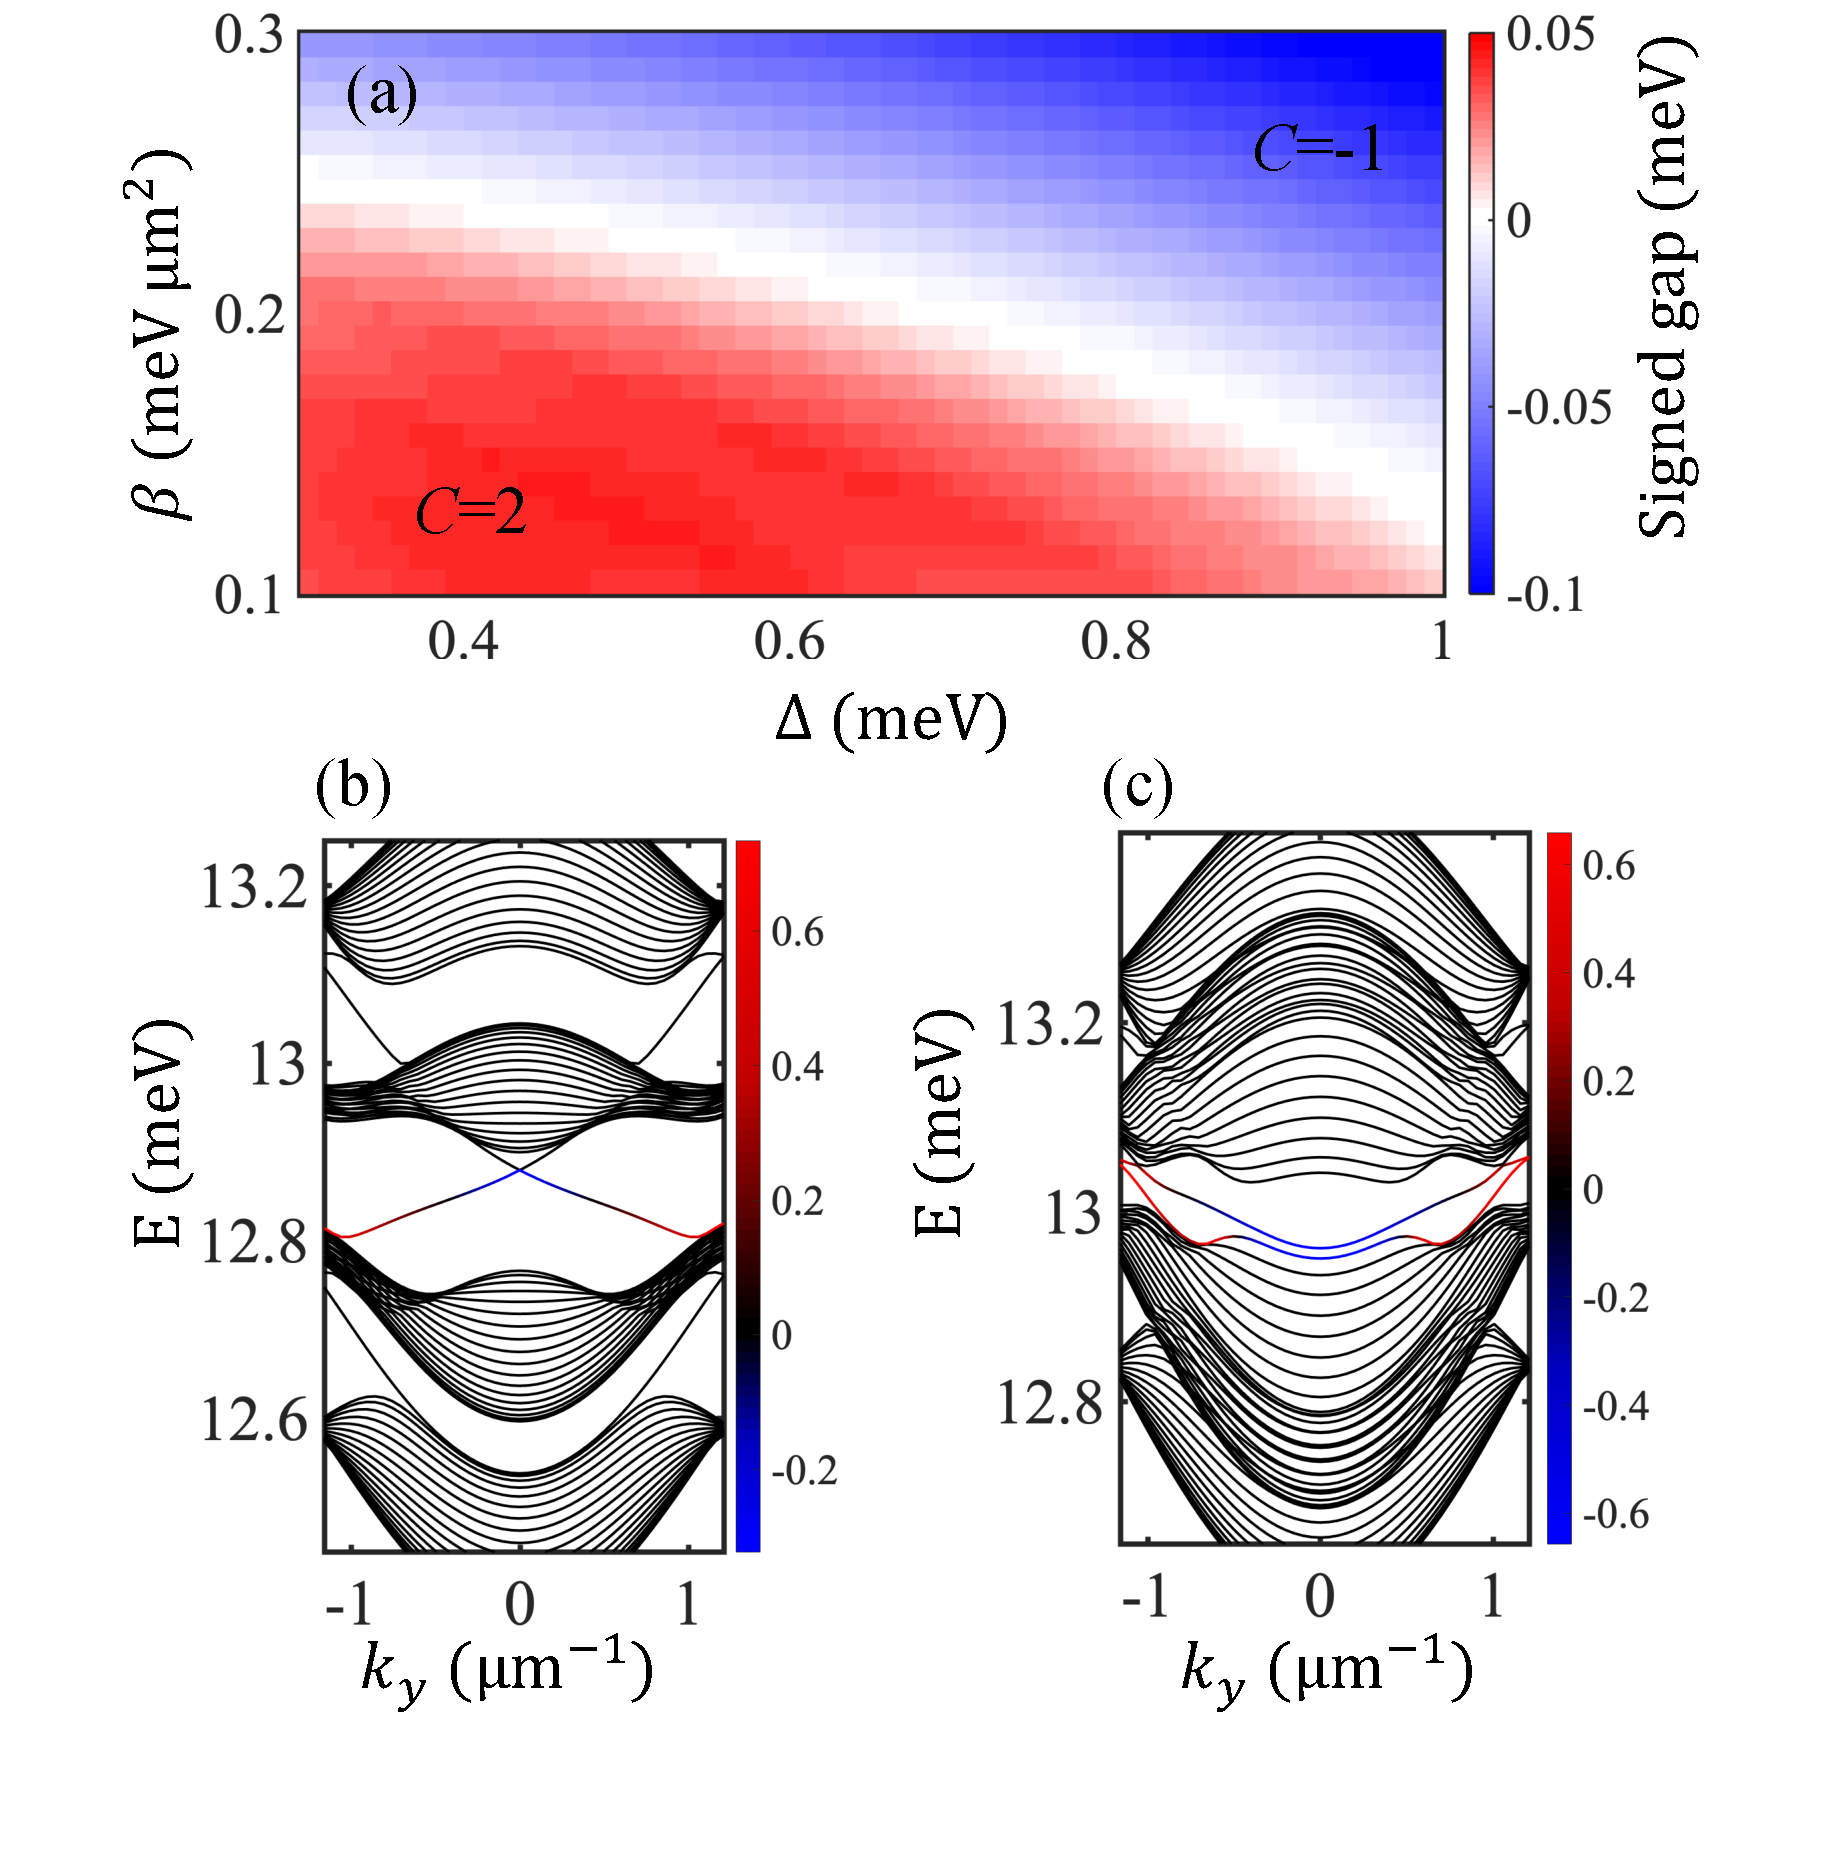
\includegraphics[height=0.98\textheight]{./fig/ch5_3.pdf}
%\end{center}
%\end{frame}

\end{document}
